% 
% Lecture Template for ME3023 -  Measurements in Mechanical Systems - Tennessee Technological University
%
% Spring 2020 - Summer 2020
% Tristan Hill, May 07, 2020 - June 12, 2020 - July 08, 2020
% Module 6->4 - Steady State Circuits
% Topic 3 - Circuit Applications
%


\documentclass[fleqn]{beamer} % for presentation (has nav buttons at bottom)

%\usepackage{/home/thill/Documents/lectures/measurements_lectures/measurements_lectures}
\usepackage{/home/tntech.edu/thill/courses/measurements/lectures/measurements_lectures}


\newcommand{\MNUM}{4\hspace{2mm}} % Module number
\newcommand{\TNUM}{3\hspace{2mm}} % Topic number 
\newcommand{\moduletitle}{Steady State Circuits}
\newcommand{\topictitle}{Circuit Applications} 

\newcommand{\sectiontitleI}{Circuits in Mechanical Engineering}
\newcommand{\sectiontitleII}{Drain Pipe Theory}
\newcommand{\sectiontitleIII}{Example 1: LED Circuit}
\newcommand{\sectiontitleIV}{Example 2: LDR circuit}

% custom box
\newsavebox{\mybox}

\title{Lecture Module - \moduletitle}

\date{Mechanical Engineering\vspc Tennessee Technological University}

\begin{document}
	
	\lstset{language=MATLAB,basicstyle=\ttfamily\small,showstringspaces=false}
	
	\frame{\titlepage \center\begin{framed}\Large \textbf{Topic \TNUM - \topictitle}\end{framed} \vspace{5mm}}


% Section 0: Outline
\frame{

\large \textbf{Topic \TNUM - \topictitle} \vspace{3mm}\\

\begin{itemize}

	\item \sectiontitleI    \vspc % Section I
	\item \sectiontitleII 	\vspc % Section II
	\item \sectiontitleIII 	\vspc % Section III
	\item \sectiontitleIV 	\vspc % Section IV

\end{itemize}

}

% Section I:
\section{\sectiontitleI}

% Section I - Frame I:
\frame{ \small
\frametitle{\sectiontitleI}

		How much does a mechanical engineer need to know about electricity and magnetism? This is good question, and obviously it varies based on your particular area of mechanical engineering. However...
	
	\begin{itemize}
		
		\item System design is integrated! Look around you, can you find anything that was developed or designed without circuits? Engineering is an integrated discipline and very few products or designs are isolated so to a single field.
		
		\item Further, the need for measurements in mechanical systems drives the need for a mechanical engineer to have a solid foundation in basic circuits theory.
			
	\end{itemize}

}

% Section I - Frame II:
\frame{
\frametitle{\sectiontitleI}

{\bf Mechatronics} \\
	Many devices or designs combine mechanical and electrical systems. This is known as Mechatronics and if you are interested in this area you are in a great place to learn. TnTech Mechanical Engineering offers a concentration in Mechatronics Engineering. In this degree you will study both mechanical engineering and electrical engineering topic to give you the foundation to design truly integrated systems! Ask me or Dr. Canfield if you have any questions about this. 

}

%% Section II:
\section{\sectiontitleII}

% Section II - Frame I:
\frame{\small
\frametitle{\sectiontitleII}

	
	{\bf Fluid Flow - Hydraulic Analogy} \vspc
	
	Traditionally engineers have used an analogy relating the movement of electrons to the flow of water through a pipe (\href{https://en.wikipedia.org/wiki/Hydraulic_analogy}{\BL hydraulic analogy}) known as {\it drain-pipe theory}. \vspace{5mm}
	
	This may provide a sense of intuition {\it however} this comparison is not accurate do to the non-Newtonian nature of electricity and magnetism (\href{https://www.slideshare.net/PDiCEOThaneHeins3240/georgia-state-university-hyperphysics-how-newtonian-mechanics-is-incorrectly-being-applied-to-explain-the-laws-of-electricity-and-magnetism}{\GR more on this}). It can  be used to visualize some basic circuits principles, but it should not be used for analysis of complex electrical systems. 

}
	


% Section III:
\section{\sectiontitleIII}

% Section III - Frame I:
\frame{
\frametitle{\sectiontitleIII}

LEDs or Light Emitting Diodes are used more and more everyday and traditional {\it incandescent} lights are used rarely in new deigns.\\
 Why are LEDs better? Can you think of any trade-offs? \\

\begin{multicols}{2}
Pros:
\begin{itemize}
\item 
\item
\item
\end{itemize}
Cons:
\begin{itemize}
\item 
\item
\item
\end{itemize}

\end{multicols}

}

% Section III - Frame II:
\frame{ \small
\frametitle{\sectiontitleIII}

\begin{multicols}{2}
An LED is designed to operate in a specific current range therefore is typically used in a voltage divider circuit that reduces the voltage across the LED so that the proper amount of current flows through the LED. Too little current not produce much light and too much current will destroy the LED or reduce the lifetime of the device.

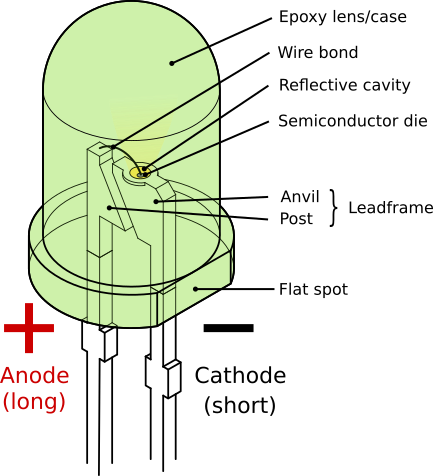
\includegraphics[scale=.4]{fancy_led.png} 

\end{multicols}


}


% Section III - Frame III:
\frame{
\frametitle{\sectiontitleIII}

Design a circuit with a voltage source, an LED, a resistor, and a SPST switch for turning on the LED. Choose the resistor such that the current is in the appropriate for a typical LED ($\sim 20mA$). The voltage drop for a green LED at $\sim 20mA$ in known to be $\sim 3.5 v$. \vspace{30mm}

}

% Section IV:
\section{\sectiontitleIV}

% Section IV - Frame I:
\frame{
\frametitle{\sectiontitleIV}
\small

Consider this circuit for measuring light intensity with an LDR (light dependent resistor). The sensors is used in a voltage divider circuit. 

\begin{multicols}{2}
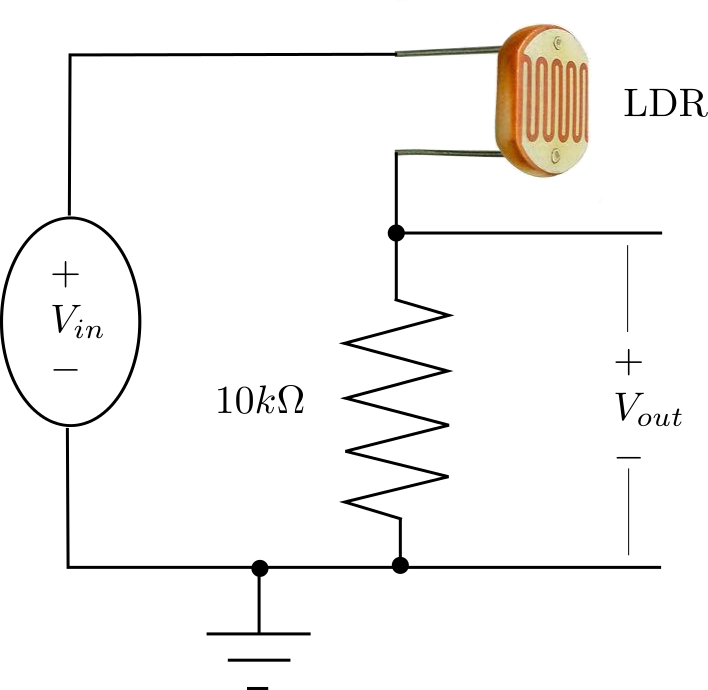
\includegraphics[scale=.20]{ldr_circuit.png}

\begin{enumerate}

\item Find the current in the circuit.
\item Find the voltage across the LDR and the $10K\Omega$ resistor.
\item Find the total energy dissipated in the circuit over 60 seconds. \vspc

\item Question: Why is the $10K\Omega$ resistor needed? 

\end{enumerate}
\end{multicols}

}
	
% Section IV - Frame II:
\frame{
\frametitle{\sectiontitleIV}
\small



}


\end{document}





